\rhead{相关概念与相关工作介绍}
\chapter{相关概念与相关工作介绍}

%@@@@@@@@@@@@@@@@@@@@@@@@@@@@@@@@@@
\section{相关概念介绍}
本章主要对本文中经常出现的一些概念作相关介绍以及形式化的定义。

\subsection{PPI网络}
蛋白质相互作用网络(protein-protein interaction networks),简称PPI网络,是一种生物体内表示蛋白质相互之间作用的图论模型。定义图$G=(V,E)$为一个PPI网络,其中$V$是点集,其中每个点$v\in V$代表一种蛋白质,$E$是一个$V×V$的边集,一条边$(u,v)\in E$代表蛋白质$u$和$v$具有相互作用。由定义可知$G$是一个\textbf{无权无向图}。
%@@@@@@@@@@@@@@@@@@@@@@@@@@@@@@@@@@@@@@@@@@@@@@@@
\subsection{全局网络匹配}
全局网络匹配(global network alignment)是对两个PPI网络$G_1(V_1,E_1)$,$G_2(V_2,E_2)$进行匹配的过程,不失一般性,$|V_1|\leq|V_2|$,并且称$G_1$为源网络(source network),$G_2$为目标网络(target network)。定义两个PPI网络$G_1,G_2$的匹配是一个从$V_1$到$V_2$的\textbf{单射}$f:V_1\rightarrow V_2$。在全局网络匹配$f$下,令$v_1\in V_1$为图$G_1$中的一个点,则$f(v_1)\in V_2$,是$v_1$在$G_2$中对应的匹配点,称$(v1,f(v1))$为一对\text{匹配点对}。由单射的定义,$G_1$的每个点都对应$G_2$中不同的点。令$f^{-1}$为$f$的反函数,由于$|V_1|\leq|V_2|$,$G_2$中可能存在没有被$G_1$中匹配到的点,可用$f^{-1}(v)=undefined$来表示。

在匹配$f$下,如果有一条源网络中的边$(u,v)\in E_1$满足$(f(u),f(v))\in E_2$,则称边$(u,v)$在$f$下是被保留(匹配)的边(conserved edge)。

令$X\subseteq V$,则$G[X]$表示图$G$中点集$X$的导出子图(induced subgraph),且$E(G[X])=\{(u,v):u\in X,v\in X,(u,v)\in E\}$表示该导出子图的边集合。

令$f(E_1)=\left \{(f(u),f(v))\in E_2:(u,v)\in E_1\right \}$,$f(V_1)=\left\{f(v)\in V_2:v\in V_1\right\}$。称$f(E_1)$为边集$E_1$在匹配$f$下的保留(匹配)边集合。它的大小衡量了$E_1$中的边在匹配后被保留下来的数量。而$f(V_1)$则是$G_2$中被匹配的点组成的集合,称为\textbf{匹配点集}。

如何衡量一个匹配的好坏,是网络匹配中一个重要的问题,因此存在许多种不同的\textbf{网络匹配衡量指标}(alignment quality measure)。
$$EC(f)=\frac{\left | f(E_1) \right |}{\left | E_1 \right |}\cite{kuchaiev2010topological}$$表示源网络$G_1$中在匹配$f$下,$E_1$中被保留下来的边数的比例,是最为常见的衡量指标。但是由于只考虑是源网络边的保留比例,在源网络是稀疏网络,目标网络是稠密网络的情况下,该指标的值会接近于1,但是并不能说明匹配的效果(虽然源网络中多数边都被保留了下来,但是目标网络中有大量的边并没有被匹配到)。
$$ICS(f)=\frac{\left | f(E_1) \right |}{\left |E_2(G_2[f(V_1)])\right |}\cite{patro2012global}$$则表示在匹配$f$下,$E_1$中被保留下来的边的数量在$G_2$中匹配点集的引导子图的边集中,所占的比例,也就是$G_2$中,被匹配点集$f(V_1)$形成的导出子图的边集中,在匹配$f$下,被匹配到的边的比例。可见与EC指标的定义恰好相反。该指标在源网络是稠密网络,目标网络是稀疏网络的时候,不能体现很好的效果。
$$TWEC(f)=\frac{EC(f)+ICS(f)}{2}\cite{dopmann2013survey}$$则平均了上面两个指标,一定程度上缓解了极端情况下衡量效果不好的情况。
$$S^{3}(f)=\frac{\left | f(E_1) \right |}{\left | E_1 \right |+\left | E_2(G_2[f(V_1)]) \right |-\left | f(E_1) \right |}\cite{saraph2014magna}$$则同时考虑了源网络和目标网络,相对EC和ICS来说是一个更好的指标。图\ref{fig:measure}展示了一个计算全局网络匹配不同衡量标准的例子。

\begin{figure}[htbp]
\centering
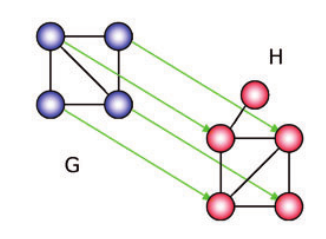
\includegraphics[height=0.25\textheight]{pic/measure.png}
\captionsetup{margin=50pt}
\caption{$G$为源网络,$H$为目标网络,其中各项指标的值分别为$EC=4/5=0.8,ICS=4/5=0.8,TWEC=0.8,S^3=4/6=0.67$ \cite{saraph2014magna} \label{fig:measure}}
\end{figure}

%@@@@@@@@@@@@@@@@@@@@@@@@@@@@@@@@@@@
\section{相关工作介绍}
到目前为止,有很多PPI网络的全局匹配算法,本文首先对主要对其中四种经典的算法进行简单的介绍,然后则介绍近年来一些文章构建动态PPI网络的方法。
%@@@@@@@@@@@@@@@@@@@@@@@@@@@@@@@@@@@@@@@@
\subsection{IsoRank算法}
IsoRank是全局网络匹配问题中被提出的第一个具有开拓性意义的算法。它主要分为两步。
第一步,IsoRank算法计算源网络$G_1$和目标网络$G_2$之间任意点对之间的相似性,用一个分数$R_{ij},i\in V_1,j\in V_2$来表示。IsoRank算法借鉴了Google的PageRank算法,任意点对$(i,j)$之间的值由$i$和$j$两个点的所有邻居节点的值所决定。见公式\ref{isorank1}的定义。

\begin{equation}\label{isorank1}
R=\sum R_{ij}=\sum_{u\in N(i),v\in N(j)}\frac{1}{\left | N(u) \right |\left | N(v) \right |}R_{uv}
\end{equation}
$N(i),N(j)$分别对应点i和点j的邻居点集。定义

\begin{equation}\label{isorank2}
A[i,j][u,v]=\begin{cases}
\frac{1}{\left | N(u) \right |\left | N(v) \right |} & \text{  } (i,u)\in E_1, (j,v)\in E_2 \\ 
 0& \text{  } \text{其他}
\end{cases}
\end{equation}
则有
\begin{equation}\label{isorank3}
R=AR
\end{equation}
从公式\ref{isorank3}可以看出,$R$是关于矩阵$A$的一个特征向量,在$A$是个稀疏矩阵的情况下,求解$A$的特征向量可以使用一种叫\textbf{幂法}(power method)的迭代方法,具体过程为:先随意初始化$R$,然后不断迭代,假设第$k$轮已经迭代完成,现在要进行第$k+1$轮迭代,则有
\begin{equation}\label{isorank4}
R(k+1)\leftarrow AR(k)/\left \|AR(k)\right \|
\end{equation}
当$\left \|R(k+1)-R(k)\right \|\rightarrow 0$时即可终止迭代。

有了$R$,第二步,就是IsoRank算法构造匹配的过程。IsoRank不断按分数从大到小挑选考查点对$(i,j)$的情况,如果当前的点对$i$和$j$都没有被匹配过($f(i)=undefined,f^{-1}(j)=undefined$),则将点对$(i,j)$作为新的\textbf{匹配点对}加入最终的匹配结果,直到不能挑出符合条件的点对为止。
IsoRank可以说是全局网络匹配算法中的一个经典算法,其经典之处在于两步走的解决问题的框架。\textbf{第一步},定义点对之间的相似度,\textbf{第二步},根据相似度按某种策略不断产生匹配点对,这一解决问题的思路为之后不少的全局网络匹配算法所采用,具有很高的开创性意义。
%@@@@@@@@@@@@@@@@@@@@@@@@@@@@@@@@@@@@@@@@@@@@@@@@@@@
\subsection{GRAAL算法}
GRAAL算法(GRAph ALigner)是一系列算法的总称,第一个提出的算法为GRAAL\cite{kuchaiev2010topological},而最近刚提出的算法为L-GRAAL\cite{malod2015graal}。这一系列算法的共同点是都使用了一种叫\textbf{小图度数}(graphlet degree)的特征作为网络中一个点的拓扑结构的度量,并且基于该度量,定义了两个不同的网络的点对之间的相似度。

一个度数为$n$的\textbf{小图}(graphlet)就是一个有$n$个点的连通图(connected graph)。图\ref{fig:graphlet}展示了所有度数在5以内(包括5)的小图,可以看到,这些小图的某些点是被标了号的,这些被标号的点被称为orbit,它们是一个小图中互相不同构的点。

\begin{figure}[htbp]
\centering
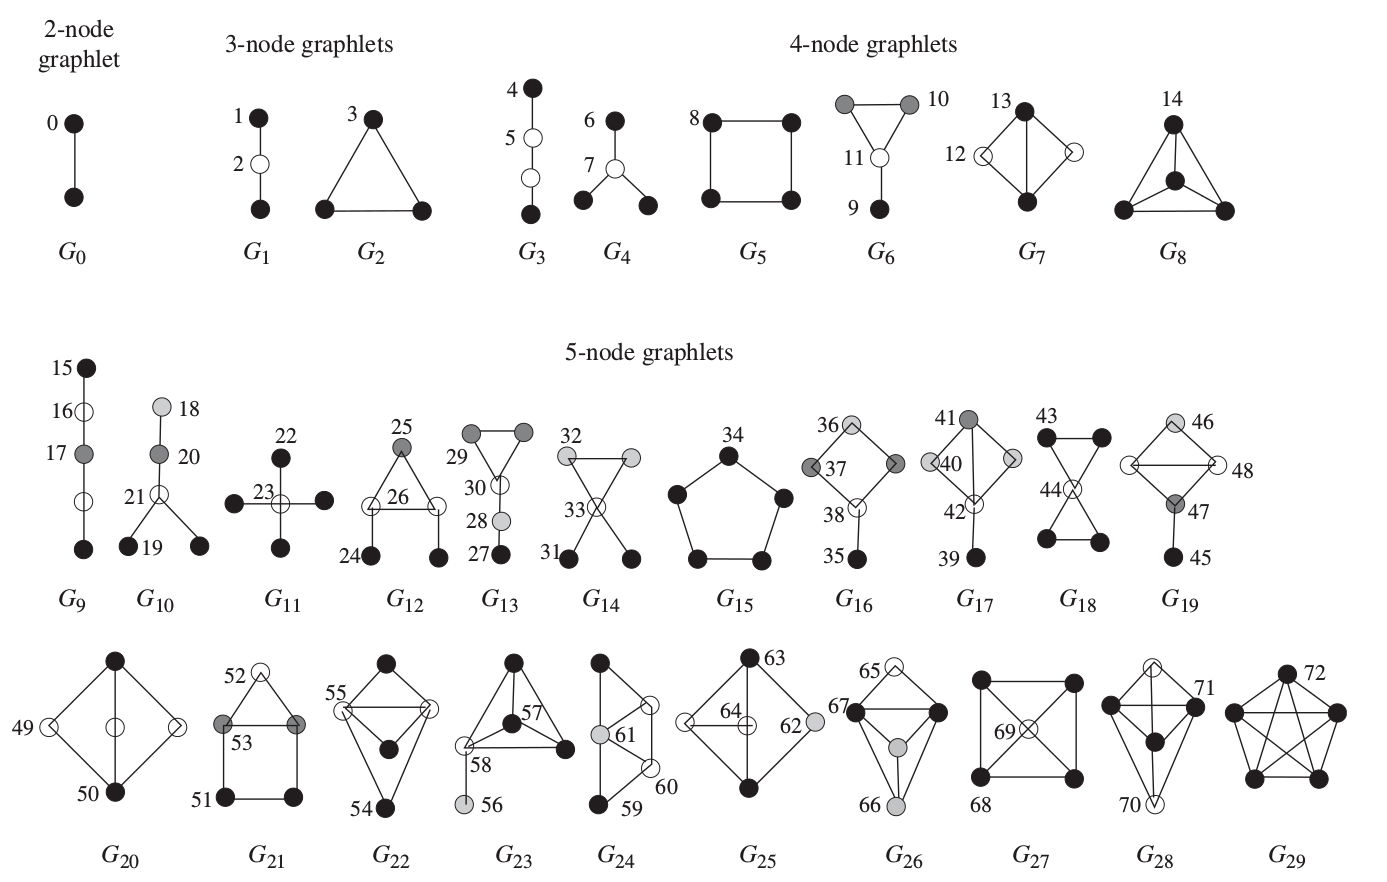
\includegraphics[width=\textwidth]{pic/graphlet.png}
\captionsetup{margin=50pt}
\caption{所有点数小于等于5的互不同构的小图\cite{kuchaiev2010topological}}\label{fig:graphlet}
\end{figure}

对于图$G$中的任意一个点$v$,它的小图度数,是一个\textbf{向量},其向量的第$i$维的值表示的就是以点$v$为中心,第$i$个orbit代表的小图出现在$v$周围的次数。形象化理解,就是将点$v$与第$i$个orbit匹配,看第$i$个orbit所在的小图是否能够匹配上以点$v$为中心延伸出去的子图,通过不同方式延伸出去得到的和小图匹配的子图分别计数,总出现次数就是第$i$维所表示的值。可见小图度数是一种可以衡量一个点周围拓扑结构的度量值。图\ref{fig:orbitcount}展示了如何衡量一个点$v$的小图度数。

\begin{figure}[htbp]
\centering
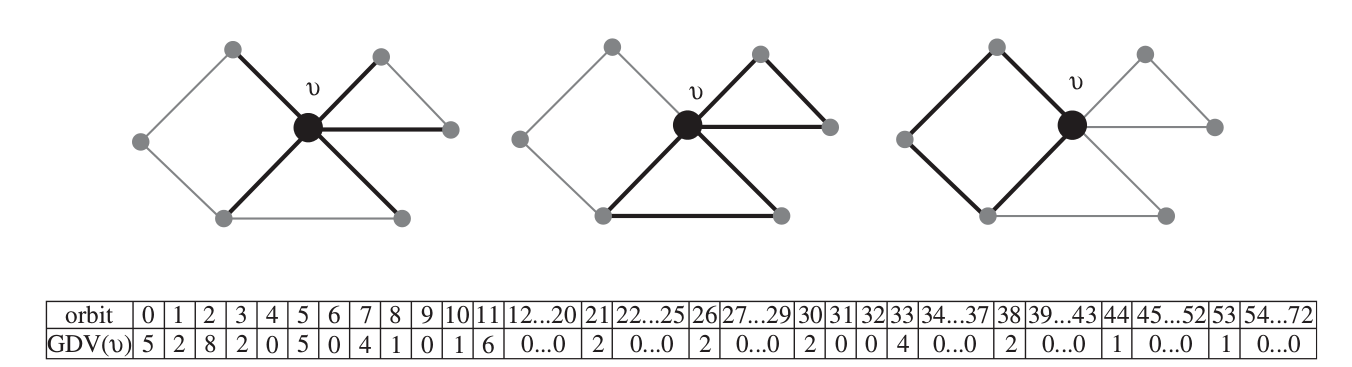
\includegraphics[width=\textwidth]{pic/orbitcount.png}
\captionsetup{margin=50pt}
\caption{点$v$的小图度数$GDV(v)\cite{kuchaiev2010topological}$}\label{fig:orbitcount}
\end{figure}

GRAAL算法,在基于小图度数这个度量值之上,定义了不同网络之间点对之间的相似度。由公式\ref{graal1}定义。

\begin{equation}\label{graal1}
S(u,v)=1-\frac{\sum_{i=0}^{72}D_i(u,v)}{\sum_{i=0}^{72}w_i}
\end{equation}

其中

\begin{equation}\label{graal2}
D_i(u,v)=\frac{w_i*\left | log(u_i+1)-log(v_i+1) \right |}{log(max\{u_i,v_i\}+2)}
\end{equation}

$u_i$和$v_i$分别是点$u$小图度数和点$v$小图度数的第$i$维向量值,$w_i$是和第$i$个orbit相关的一个权重。

在有了相似度函数以后,GRAAL也和IsoRank一样,通过相似度函数,设计了一种生成匹配点对的策略。然而不同于IsoRank的策略,GRAAL采取的策略是,每次挑选出一对还没匹配过的点对$(i,j)$,称为种子点对(seed pair),然后考查任意一对由$i$的邻居点集$N(i)$的点和$j$的邻居点集$N(j)$中的点组成的点对$(u,v),u\in N(i),v\in N(j)$。将这些考查的点对根据相似度大小贪心的进行匹配,当不存在能匹配的点对的时候,GRAAL才继续寻找下一个种子点对,这是和IsoRank不同的地方。可以说GRAAL算法寻找匹配的策略是先全局,再局部的策略。

GRAAL系列之后又出现了H-GRAAL\cite{milenkovic2010optimal},MI-GRAAL\cite{kuchaiev2011integrative},C-GRAAL\cite{memivsevic2012c}和L-GRAAL\cite{malod2015graal}。而最近提出的L-GRAAL\cite{malod2015graal}算法,通过解线性规划的问题来进行匹配,显示出了极好的匹配效果。

%@@@@@@@@@@@@@@@@@@@@@@@@@@@@@@@@@@@@@@@@@@@@@@@@@@@@@@@@@@@@@@@@@@@@@@
\subsection{SPINAL算法}
SPINAL算法(scalable protein interaction network alignment)也是类似于IsoRank和GRAAL的算法。它也是分两步走的框架。第一步,定义节点之间的相似度$P(i,j)$,并且与IsoRank类似的,它采用不断迭代的方式不断更新$P$的值,$P$的初始值由两个节点之间的度数差决定

\begin{equation}\label{spinal1}
P(i,j)=DegDiff(i,j)
\end{equation}

每一轮迭代,$P(i,j)$的值由i和j的邻居点集$N(i)$和$N(j)$决定,但是SPINAL算法采用了与IsoRank算法不同的计算公式。

定义$NBG(\left \{ \left \langle i,j \right \rangle \right \},P)$为一个\textbf{二分图}(bipartite graph),其中二分图左边的顶点集合$X$由点$i$的邻居集合$N(i)$构成($X=N(i)$),右边的顶点集合$Y$由点$j$的邻居集合$N(j)$构成($Y=N(j)$),任意一条二分图中的边$(x,y)\in NBG,x\in X,y\in Y$,边权$w(x,)=P(x,y)$。

每一轮迭代更新点对$(i,j)$,SPINAL算法使用不同于IsoRank算法的计算方法:首先构造出二分图$NBG(\left \{ \left \langle i,j \right \rangle \right \},P)$,然后得到$NBG$的\textbf{最大权值匹配}(maximum weighted bipartite matching)。令得到的匹配边集合为$C$,称为贡献者集合(contributors set),则新的$P(i,j)$值为

\begin{equation}\label{spinal2}
P(i,j)=\frac{\sum_{(x_i,y_j)\in C}\frac{P(x_i,y_j)}{deg(x_i)*deg(y_j)}}{\sqrt{\left | C \right |}}
\end{equation}
若干轮迭代后,就能得到最后的相似度矩阵$P$了。

SPINAL算法的第二步则是基于$P$矩阵的值,产生匹配点对的过程,和GRAAL算法类似。SPINAL先将所以的匹配点对按照$P$值从大到小排序,每次挑选出一对还未得到匹配的种子点对$(i,j)$,然后构造二分图$NBG(\left \{ \left \langle i,j \right \rangle \right \},P)$,求出该二分图的最大权值匹配边集合$M$。之后,SPINAL会重新依次检查二分图中的每一条非匹配边(不在集合$M$中),看看是否能够通过交换这条非匹配边与$M$中的匹配边得到更优的匹配。这相当于是一个局部调优的过程。经过调优过程以后,将得到的所有的匹配边,都当做是新的匹配点对加入到当前的匹配点对集合中。然后再去寻找新的满足条件的种子点对,进行下一轮的局部调优过程,直到不存在种子点对为止。

SPINAL算法的精髓在于将匹配点对的邻居之间的关系用二分图最大权值匹配这一模型表达了出来,同时利用局部调优的策略来产生更好的解。
%@@@@@@@@@@@@@@@@@@@@@@@@@@@@@@@@@@@@@@@@@@@@@@@@@@@@@@@@@@@@@@@@@@@@
\subsection{PROPER算法}
PROPER算法(PROtein-protein interaction network alignment based on PERcolatin)\cite{kazemi2016proper}是一种基于\textbf{图渗透}的PPI网络匹配算法。不同于之前三个算法的是,PROPER算法并没有将过多的重点放在计算两个网络之间任意点对之间的相似度上。PROPER算法对于两个待匹配的PPI网络,用点对所代表的蛋白质间的BLAST分数\cite{altschul1990basic}(一种衡量蛋白质序列之间相似度的分数)作为这两个网络任意点对之间的相似度函数,即

\begin{equation}\label{proper1}
S(i,j)=BLAST\_SCORE(i,j)
\end{equation}

PROPER算法认为,当两个蛋白质的BLAST分数较大的时候,意味着它们之间的序列相似度很高,那么这两个蛋白质,在它们的功能表达上,相似的概率也应该是很大的,虽然像之前说的,考虑到蛋白质之间的相互作用,光是序列的相似性,并不能代表它们在网络中和其他蛋白质相互作用的相似性,但是PROPER认为,如果这样的相似度高于一个阈值,则可以认为它们在PPI网络中,也拥有相似度极高的网络结构,因此,可以先找出所有这样的点对,将它们进行匹配,产生一个点对匹配的集合,也略去了利用网络结构计算点对间相似性的过程。这也是PROPER算法的第一步。而PROPER算法的精髓在其第二步。

PROPER算法的第一步,如前文所说,按照BLAST分数作为相似度衡量指标,将所以待匹配点对按值从大到小进行排序。然后依次考虑每一对待匹配的点对$(i,j):S(i,j)\geq l$,将$(i,j)$加入集合$A$,直到没有符合条件的点对为止。最后得到的集合$A$就是PROPER算法第一步产生的匹配点对集合。

$l$是PROPER算法第一步的一个参数,阈值$l$越小,满足条件的待匹配点对便越多,第一步中被加入$A$的匹配点对就越多。也就是说,第一步产生的匹配只是部分匹配,而其大小则取决于参数$l$的值。

PROPER算法的第二步是在第一步结果$A$的基础上,扩展匹配点对的过程(图渗透算法)。定义
\begin{equation}\label{proper2}
F_A(i,j)=\left | \{(u,v):u\in N(i),v\in N(j),(u,v)\in A\} \right |
\end{equation}
称为点对$(i,j)$在已有匹配$A$下的贡献值。$F_A(i,j)$的实际意义在于,源网络$G_1$在已有匹配$A$的情况下,通过新增一对匹配点对$(i,j)$,此时在新的匹配$A\bigcup \{(i,j)\}$的情况下,$E_1$中能够增加的被匹配(保留)的边数。根据前面定义的四种匹配衡量标准,可以认为$E_1$中被保留的边越多,则匹配越好。PROPER算法的第二步,便是将所有$F_A\geq r$且没有被匹配过的点对,按照$F_A$的值进行排序,挑选其中最好的一对加入集合$A$的过程。在集合$A$变化了以后,所有点对的$F_A$值重新计算,重新排序,重新挑选,这就是图渗透的过程。

从PROPER算法的过程可以看到阈值$l$和$r$对PROPER算法有着极为重要的意义和影响,阈值$l$影响集合$A$的大小,而$r$影响的是第二步中可以新加入$A$的匹配点对的数量。因此$l$和$r$分别控制了蛋白质序列相似度和网络结构相似度对整个算法的影响比例。

%@@@@@@@@@@@@@@@@@@@@@@@@@@@@@@@@@@@@@@@@@@@@@@@@@@@@@@@@@@@@@@@@@@@
\subsection{动态PPI网络生成}
本来,所有的PPI网络数据都是静态的,如何将PPI网络构造成动态的呢?\cite{zhang2016method}给出了一种合理的动态PPI网络构造方法。

\textbf{基因表达数据}(gene expression data)是对一个蛋白质在生物细胞作用中表现出来的基因水平提供衡量指标的数据。通过基因表达数据,我们可以很容易的知道生物体中的每一个蛋白质,在细胞生命活动的各个阶段,所表现出来的基因表达水平(gene expression level)分别是多少。在细胞生命活动中,一种蛋白质的基因表达水平与它在该生命活动中所起到的作用成\textbf{正相关}关系。因此,一个简单的想法就是,通过查看一个蛋白质的各个时刻的基因表达水平,来判断它在哪些时刻是处于活跃状态,哪些时刻是处于不活跃状态的。

定义一个蛋白质的基因表达数据为

\begin{equation}\label{dppi1}
p=[ p_1,p_2,p_3,....,p_n]
\end{equation}
$p$是一个数值序列,其中$p_i$为该蛋白质在$i$时刻的基因表达水平。\cite{zhang2016method}使用了一种三-西格玛阈值的方法来确定一个蛋白质何时处于活跃阶段,何时处于不活跃阶段。定义

\begin{equation}\label{dppi2}
Thresh_k(p)=\alpha (p)+k*\sigma (p)*\left (1-\frac{1}{1+\sigma ^2(p)}\right )
\end{equation}
为该蛋白质基因表达数据的三-西格玛阈值($k=1,2,3$)。其中$\alpha (p)$为$p$序列的平均值,$\sigma (p)$为标准差。

如果把$p$序列看成一个服从正态分布$N(\alpha,\sigma)$的随机变量,那么可以知道,$P(|X-\alpha|<\sigma)\approx 0.6827,P(|X-\alpha|<2\sigma)\approx 0.9545,P(|X-\alpha|<3\sigma)\approx 0.9973$。定义

\begin{equation}\label{dppi3}
Pr_i(p)= \begin{cases}
0.99 & \text{  } p_i\geq Thresh_3(p)\\ 
0.95 & \text{  } Thresh_3(p)> p_i\geq Thresh_2(p) \\ 
0.68 & \text{  } Thresh_2(p)> p_i\geq Thresh_1(p) \\ 
0 & \text{  } p_i<Thresh_1(p) 
\end{cases}
\end{equation}


为蛋白质在$i$时刻活跃的概率。通过这个方法,我们可以算出一个PPI网络中,所有蛋白质在每个时刻的活跃概率。我们认为两个蛋白质之间的相互作用,只有当这两个蛋白质都处于活跃状态时才有意义,那么

\begin{equation}\label{dppi4}
Pr_i((u,v))= Pr_i(u)*Pr_i(v)
\end{equation}
就是边$(u,v)$在$i$时刻活跃的概率。

如果一个PPI网络在一个很长的时间序列内不断变化,假设这样的时间序列长度为T(即有T个时刻),那么,一个静态的PPI网络就可以转化成一个动态PPI网络,该动态PPI网络由T个静态PPI网络组成,其中每个静态PPI网络的点和边都有不同的活跃概率。图\ref{fig:dppi}展示了一个动态PPI网络的例子。可以看到该动态PPI网络由三个静态PPI网络构成,每一个静态PPI网络中的点和边都不同,意味着每个时刻动态PPI网络都是不同的。

\begin{figure}[htbp]
\centering
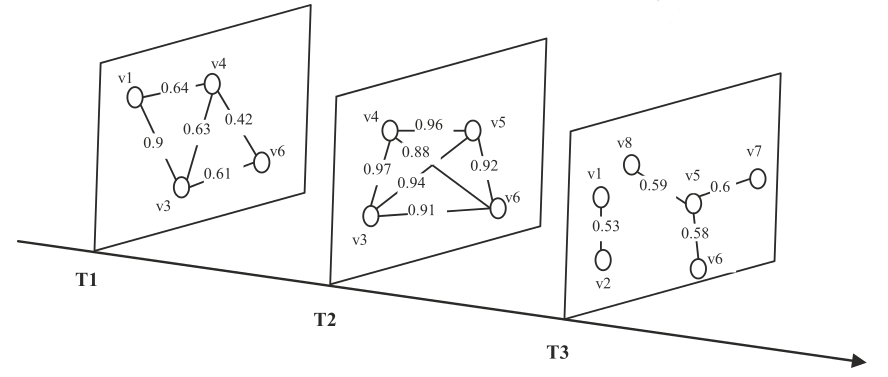
\includegraphics[height=0.25\textheight]{pic/dppi.png}
\captionsetup{margin=50pt}
\caption{动态PPI网络 \cite{zhang2016method} \label{fig:dppi}}
\end{figure}
